\documentclass[10pt,leter,openany]{article}
\usepackage[latin1]{inputenc}
\usepackage[english]{babel}
\usepackage{amsmath}
\usepackage{amsfonts}
\usepackage{amssymb}
\usepackage{graphicx}
\usepackage{listings}
\usepackage{color}
\usepackage[left=3cm,right=3cm,top=3cm,bottom=3cm]{geometry}
\usepackage[numbers,sort&compress]{natbib}
\usepackage{url}
\usepackage{caption}
\usepackage{siunitx}
%\usepackage{subfigure}
\usepackage{float}
\usepackage{booktabs}
\usepackage{subcaption}
\usepackage{comment}
\usepackage{mwe}
%\usepackage[table,xcdraw]{xcolor}
\usepackage[shortlabels]{enumitem}   %To enumerate with letters
\usepackage{mathtools}	%To write derivates
\usepackage[thinc]{esdiff}	%To write derivates
\usepackage{cancel} %To cancel terms in equations

\setlength{\parindent}{0pt}
\setlength{\parskip}{4pt}

\definecolor{mygreen}{rgb}{0,0.6,0}
\definecolor{mygray}{rgb}{0.5,0.5,0.5}
\definecolor{mymauve}{rgb}{0.58,0,0.82}

\lstset{ 
	backgroundcolor=\color{white},   % choose the background color; you must add \usepackage{color} or \usepackage{xcolor}; should come as last argument
	basicstyle=\footnotesize,        % the size of the fonts that are used for the code
	breakatwhitespace=false,         % sets if automatic breaks should only happen at whitespace
	breaklines=true,                 % sets automatic line breaking
	captionpos=b,                    % sets the caption-position to bottom
	commentstyle=\color{mygreen},    % comment style
	deletekeywords={...},            % if you want to delete keywords from the given language
	escapeinside={\%*}{*)},          % if you want to add LaTeX within your code
	extendedchars=true,              % lets you use non-ASCII characters; for 8-bits encodings only, does not work with UTF-8
	firstnumber=01,                	 % start line enumeration with line 1000
	frame=single,	                 % adds a frame around the code
	keepspaces=true,                 % keeps spaces in text, useful for keeping indentation of code (possibly needs columns=flexible)
	keywordstyle=\color{blue},       % keyword style
	language=Python,                 % the language of the code
	morekeywords={*,...},            % if you want to add more keywords to the set
	numbers=left,                    % where to put the line-numbers; possible values are (none, left, right)
	numbersep=5pt,                   % how far the line-numbers are from the code
	numberstyle=\tiny\color{mygray}, % the style that is used for the line-numbers
	rulecolor=\color{black},         % if not set, the frame-color may be changed on line-breaks within not-black text (e.g. comments (green here))
	showspaces=false,                % show spaces everywhere adding particular underscores; it overrides 'showstringspaces'
	showstringspaces=false,          % underline spaces within strings only
	showtabs=false,                  % show tabs within strings adding particular underscores
	stepnumber=1,                    % the step between two line-numbers. If it's 1, each line will be numbered
	stringstyle=\color{mymauve},     % string literal style
	tabsize=2,	                     % sets default tabsize to 2 spaces
	title=\lstname                   % show the filename of files included with \lstinputlisting; also try caption instead of title
}

\usepackage[dvipsnames,table,xcdraw]{xcolor}

\usepackage{fancyvrb}

% redefine \VerbatimInput
\RecustomVerbatimCommand{\VerbatimInput}{VerbatimInput}%
{fontsize=\footnotesize,
	%
	frame=lines,  % top and bottom rule only
	framesep=2em, % separation between frame and text
	rulecolor=\color{Gray},
	%
	label=\fbox{\color{Black}data.txt},
	labelposition=topline,
	%
	commandchars=\|\(\), % escape character and argument delimiters for
	% commands within the verbatim
	commentchar=*        % comment character
}



\usepackage{titling}
\newcommand{\subtitle}[1]{%
	\posttitle{%
		\par\end{center}
	\begin{center}\large#1\end{center}
	\vskip0.5em}%
}


\author{5273}
\title{Homework Assignment 9: Applied Probabilistic Models}
\subtitle{Expected Value and Variance}
\date{}


\begin{document}
	
\maketitle

\section{Exercises}
	
	Exercises solved in this work are provided on the book \citet{grinstead2012introduction}. 
	
	\subsection{Expected Value of Discrete Random Variables}
	
	For this exercises the expected value and the variance of discrete random variables are discussed.
	
	\subsubsection*{Exercise 1 page 247}
	
	As the deck consists of cards between 2 through 10, it will have 36 cards. Let $ X $ be the number of the selected card. The player will win a dollar if the number of the card is odd and loses one dollar if the number is even, so the expected value of his winnings will be:
	
	\begin{equation*}
		E(X) = -1\left( \dfrac{4}{36}\right)  + 1\left( \dfrac{4}{36}\right)  - 1\left( \dfrac{4}{36}\right) + 1\left( \dfrac{4}{36}\right) - 1\left( \dfrac{4}{36}\right) + 1\left( \dfrac{4}{36}\right) - 1\left( \dfrac{4}{36}\right) + 1\left( \dfrac{4}{36}\right) - 1\left( \dfrac{4}{36}\right) = -\dfrac{1}{9}.
	\end{equation*}
	
	\subsubsection*{Exercise 15 page 249}
	
	In this exercise, the game stops whenever it is one dollar profit or run out of gold balls.  For one gold ball, a player wins one dollar and loses one dollar if a silver ball is drawn as the box contains two gold balls and three silver balls and let $ X $ be the results of the draws until the game is finished. There are seven possible outcomes, which are detailed below with its corresponding probability. Therefore, the expected value is:
	
	% Please add the following required packages to your document preamble:
	% \usepackage{booktabs}
	\begin{table}[]
		\centering
		\caption{Possible outcomes for Exercise 15 page 249.}
		\label{tab:ex15p247}
		\begin{tabular}{@{}lcr@{}}
			\toprule
			\textbf{Outcome} & \multicolumn{1}{l}{\textbf{Probability}} & \multicolumn{1}{l}{\textbf{Profit}} \\ \midrule \vspace{0.3cm} 
			G                &$  \left(  \frac{2}{5}       \right)       $                          & 1                                   \\ \vspace{0.3cm} 
			SGG              & $\left( \frac{3}{5}\right) \left( \frac{1}{2}\right) \left( \frac{1}{3}\right) $                                                 & 1                                   \\ \vspace{0.3cm} 
			SGSG             & $\left( \frac{3}{5}\right) \left( \frac{1}{2}\right) \left( \frac{2}{3}\right) \left( \frac{1}{2}\right) $                                         & 0                                   \\ \vspace{0.3cm} 
			SSGG             & $\left( \frac{3}{5}\right) \left( \frac{1}{2}\right) \left( \frac{2}{3}\right) \left( \frac{1}{2}\right) $                                         & 0                                   \\ \vspace{0.3cm} 
			SSSGG            & $\left( \frac{3}{5}\right) \left( \frac{1}{2}\right) \left( \frac{1}{3}\right) \left( 1\right) \left( 1\right) $                                        & -1                                  \\ \vspace{0.3cm} 
			SGSSG            & $\left( \frac{3}{5}\right) \left( \frac{1}{2}\right) \left( \frac{2}{3}\right) \left( \frac{1}{2}\right) $                                       & -1                                  \\ \vspace{0.3cm} 
			SSGSG            & $\left( \frac{3}{5}\right) \left( \frac{1}{2}\right) \left( \frac{2}{3}\right) \left( \frac{1}{2}\right) $                                        & -1                                  \\ \bottomrule
		\end{tabular}
	\end{table}
	
	\begin{equation*}
		E(X) = 1\left( \dfrac{2}{5}\right)  + 1\left( \dfrac{1}{10}\right)  + 0\left( \dfrac{1}{10}\right) + 0\left( \dfrac{1}{10}\right) -1\left( \dfrac{1}{10}\right) - 1\left( \dfrac{1}{10}\right) -1\left( \dfrac{1}{10}\right)  = \dfrac{2}{10} = \dfrac{1}{5}.
	\end{equation*}

	Because $E(X) >0$ it can be said this is a favorable game.
	
	\subsubsection*{Exercise 18 page 249}
	
	Six similar keys are given, and let $ X $ be the number of tried keys before the success of opening the door.
	\begin{equation*}
		E(X) =
		0\left( \dfrac{1}{6}\right)   + 1\left( \dfrac{1}{6}\right) +2\left( \dfrac{1}{6}\right) + 3\left( \dfrac{1}{6}\right) + 4\left( \dfrac{1}{6}\right)  +5\left( \dfrac{1}{6}\right)   = \dfrac{5}{2}.
	\end{equation*}


\subsubsection*{Exercise 19 page 249}

For every correct answer, the student gets three points and for every incorrect one loses one point. The problem has four possible answers. Let $ X $ be the result if the answer is correct or incorrect. Therefore, the probability of choosing the correct answer just guessing is 0.25, whereas the probability of choosing the incorrect one is 0.75. The expected value is:

\begin{equation*}
	E(X) = 3(0.25) -1(0.75)  = 0.
\end{equation*}

\subsubsection*{Exercise 31 page 254}

\begin{enumerate}[(a)]
	\item For a pooled sample of $ k $ people, if the test is positive, it means that each person has a positive result on the test independently with probability $p$. Therefore, the probability that each person has a negative result is $1-p$. The probability that all of the $k$ subjects have negative result is $ (1-p)^{k} $. Consequently:
	\begin{equation*}
		\begin{aligned}
			P(\mbox{sample is positive}) & = 1- P(\mbox{all \textit{k} subjects have negative results}),\\
			& = 1-(1-p)^{k}.\\
		\end{aligned}	
	\end{equation*}

\item Let $X$ be the number of blood tests necessary under the plan (2). There are $\dfrac{N}{k} $ groups of $ k $ individuals. For each of these groups, if someone is positive, a $k+1$ tests are needed, and otherwise, only one test. The expected value for the number of tests for one group is:
\begin{equation*}
	(k+1)P(Positive) + 1*P(Negative) = (k+1)(1-(1-p)^k) + 1(1-p)^k,
\end{equation*}

For the whole group of $ N $ subjects is:
\begin{equation*}
	\begin{aligned}
		E(X) & = \dfrac{N}{k}\left[ (k+1)(1-(1-p)^k) + 1(1-p)^k\right] \\
		& = \dfrac{N}{k}\left[ (k+1)-(k+1)(1-p)^k + (1-p)^k\right]\\
		& = \dfrac{N}{k}\left[ k+1-k(1-p)^k - (1-p)^k + (1-p)^k \right]\\
		& = \dfrac{N}{k}\left[ k+1-k(1-p)^k\right].\\
	\end{aligned}	
\end{equation*}

\item To minimize the expected value, it can be calculated the derivate of with respect to $ k $ and set equal to 0.
\begin{equation*}
E(k)	= \dfrac{N}{k}\left[ k+1-k(1-p)^k\right],\\
\end{equation*}

\begin{equation*}
	\begin{aligned}
	\diff{E}{k}& = 0\\
	\dfrac{-n\ln(1-p)(1-p)^k k^2+N}{k^2}& = 0,
\end{aligned}	
\end{equation*}

If in the expression above, a sufficient small $p$ is considered approximately 0, the equality would be:
\begin{equation*}
	\begin{aligned}
		\dfrac{\cancelto{0}{-n\ln(1-p)(1-p)^k k^2}+N}{k^2}& = 0\\
		\dfrac{N}{k^2}&=0,
	\end{aligned}	
\end{equation*}

When substituting the value of $ k $ to $\dfrac{1}{\sqrt{p}}$:
\begin{equation*}
	\begin{aligned}
		\dfrac{N}{k^2}& = 0\\
		\dfrac{N}{\left( \dfrac{1}{\sqrt{p}}\right) ^2}&=0\\
		\dfrac{N}{\left( \dfrac{1}{p}\right) } & =0\\
		Np & =0.
	\end{aligned}	
\end{equation*}

At this point, if the value of $p$ is sufficient small (approximately 0), the equality is fullfilled for a value of $k=\dfrac{1}{\sqrt{p}} $, where the expected number of test is minimum.

\end{enumerate}

\subsubsection*{Exercise 1 page 263}

If $\left\lbrace S=-1,0,1\right\rbrace :$

\begin{itemize}
	\item The expected value would be:
	\begin{equation*}
		E(X) = \dfrac{\sum(x)}{N} = -1\left( \dfrac{1}{3}\right)  + 0\left( \dfrac{1}{3}\right) +1\left( \dfrac{1}{3}\right) = 0.
	\end{equation*}

\item To calculate the variance it can be used Table \ref{tab:ex1p263}. Then, the variance would be:
\begin{equation*}
	\sigma^2 = \dfrac{\sum\left( x-\bar{x}\right) ^2}{N} = \dfrac{\left( -1-0\right) ^2 + \left( 0-0\right) ^2 + \left( 1-0\right) ^2}{3} = \dfrac{2}{3}.
\end{equation*}

% Please add the following required packages to your document preamble:
% \usepackage{booktabs}
\begin{table}[]
	\centering
	\caption{Variance in Exercise 1 page 263.}
	\label{tab:ex1p263}
	\begin{tabular}{@{}rrr@{}}
		\toprule
		$x $                              &  $x-\bar{x}$        & $\left( x-\bar{x}\right) ^2$            \\ \midrule
		-1                                          & -1                   & 1                          \\
		0                                           & 0                    & 0                          \\
		1                                           & 1                    & 1                          \\ \midrule
		\multicolumn{1}{c}{$\sum x_{i} = 0$} & \multicolumn{1}{c}{} & \multicolumn{1}{c}{$\sum \left( x_{i}-\bar{x} \right)^2 = 2$} \\ \bottomrule
	\end{tabular}
\end{table}

\item The standard deviation $ \sigma = \sqrt{\sigma^2}= \sqrt{\dfrac{2}{3}} \approx 0.816.$ 
\end{itemize}

	\subsection{Expected Value of Continuous Random Variables}
	
	This section corresponds to exercises of expected value and variance of continuous random variables.
	
	\subsubsection*{Exercise 3 page 278}
	
	The expected value of a continuous random variable is given by
	\begin{equation*}
		\begin{aligned}
			E(X) & = \int_{-\infty}^{\infty} x f(x)  dx,\\
		\end{aligned}	
	\end{equation*}
	
	
	Therefore the expected lifetime of the light bulb would be:
	\begin{equation*}
		\begin{aligned}
			E(T) & = \int_{0}^{\infty} t (\lambda)^2 t e^{-\lambda t}  dt\\
\lambda^2 \int t^2 e^{-\lambda t} dt&	= \lambda^{2}\left( \dfrac{-t^{2}e^{-\lambda t}}{\lambda} - \int \dfrac{-2te^{-\lambda t}}{\lambda}dt\right) \\
 & = \lambda^{2}\left[ \dfrac{-t^{2}e^{-\lambda t}}{\lambda} + \dfrac{2}{\lambda}\left( - \dfrac{te^{-\lambda t}}{\lambda} - \int \dfrac{-e^{-\lambda t}}{\lambda}dt\right) \right] \\
 & = \lambda^{2}\left[ \dfrac{-t^{2}e^{-\lambda t}}{\lambda} + \dfrac{2}{\lambda}\left( - \dfrac{te^{-\lambda t}}{\lambda} + \dfrac{1}{\lambda}\left[ \dfrac{-e^{-\lambda t}}{\lambda}\right] \right) \right] \\
 & = \left[ \dfrac{\left( -t^{2} \lambda^{2} - 2t\lambda -2\right) e^{-\lambda t}}{\lambda} \right]^{\infty}_{0}\\
 & = \dfrac{2}{\lambda}\\
 & = 40.
			\end{aligned}	
	\end{equation*}

	The variance would be:
		\begin{equation*}
		\begin{aligned}
	\lambda^2 \int t^3 e^{-\lambda t} dt&	= \lambda^{2}\left( \dfrac{-t^{3}e^{-\lambda t}}{\lambda} - \int \dfrac{-3t^{2}e^{-\lambda t}}{\lambda}dt\right) \\
	& = \lambda^{2}\left[ \dfrac{-t^{3}e^{-\lambda t}}{\lambda} + \dfrac{3}{\lambda}\left( - \dfrac{t^{2}e^{-\lambda t}}{\lambda} - \dfrac{2 t e^{-\lambda t}}{\lambda^{2}} - \dfrac{2e^{\lambda t}}{\lambda^{3}}\right) \right] \\
	& = \left[ \dfrac{\left( -t^{3}\lambda^{3} - 3t^{2}\lambda^{2} - 6t\lambda-6\right) e^{-\lambda t}}{\lambda^{2}} \right] ^{\infty}_{0}\\
	 & = \dfrac{6}{\lambda^{2}}\\
	& = 2400,
				\end{aligned}	
\end{equation*}

\begin{equation*}
	\begin{aligned}
		V(T) & = E(X^{2} - E(X)^{2})\\
		& = 2400 - 1600\\
		& = 800.
	\end{aligned}	
\end{equation*}


\subsubsection*{Exercise 12 page 280}

The variables $ X $ and $ Y $ are independent, and both are uniformly distributed on $\left[ 0,1\right]$.  The expected value of both variables is given by:

	\begin{equation*}
	\begin{aligned}
		E(X^{Y}) & = \int_{0}^{1}\int_{0}^{1} x ^{y}f(x)f(y)  dx dy\\
		& = \int_{0}^{1} \left[ \dfrac{x^{y+1}}{y+1}\right] ^{1}_{0} dy\\
		& = \int_{0}^{1} \dfrac{1}{y+1} dy\\
		& = \left[ \ln (y+1) \right] ^{1}_{0}\\
		& = \ln 2\\
		& \approx 0.6931.
	\end{aligned}	
\end{equation*}

Results of the simulation are shown in Figure \ref{fig:hist12p280}. It is performed in R software in its version 4.0.2 \citep{r}, and the code used is available on the GitHub repository of \citep{github}.

	\begin{figure}
	\begin{center}
		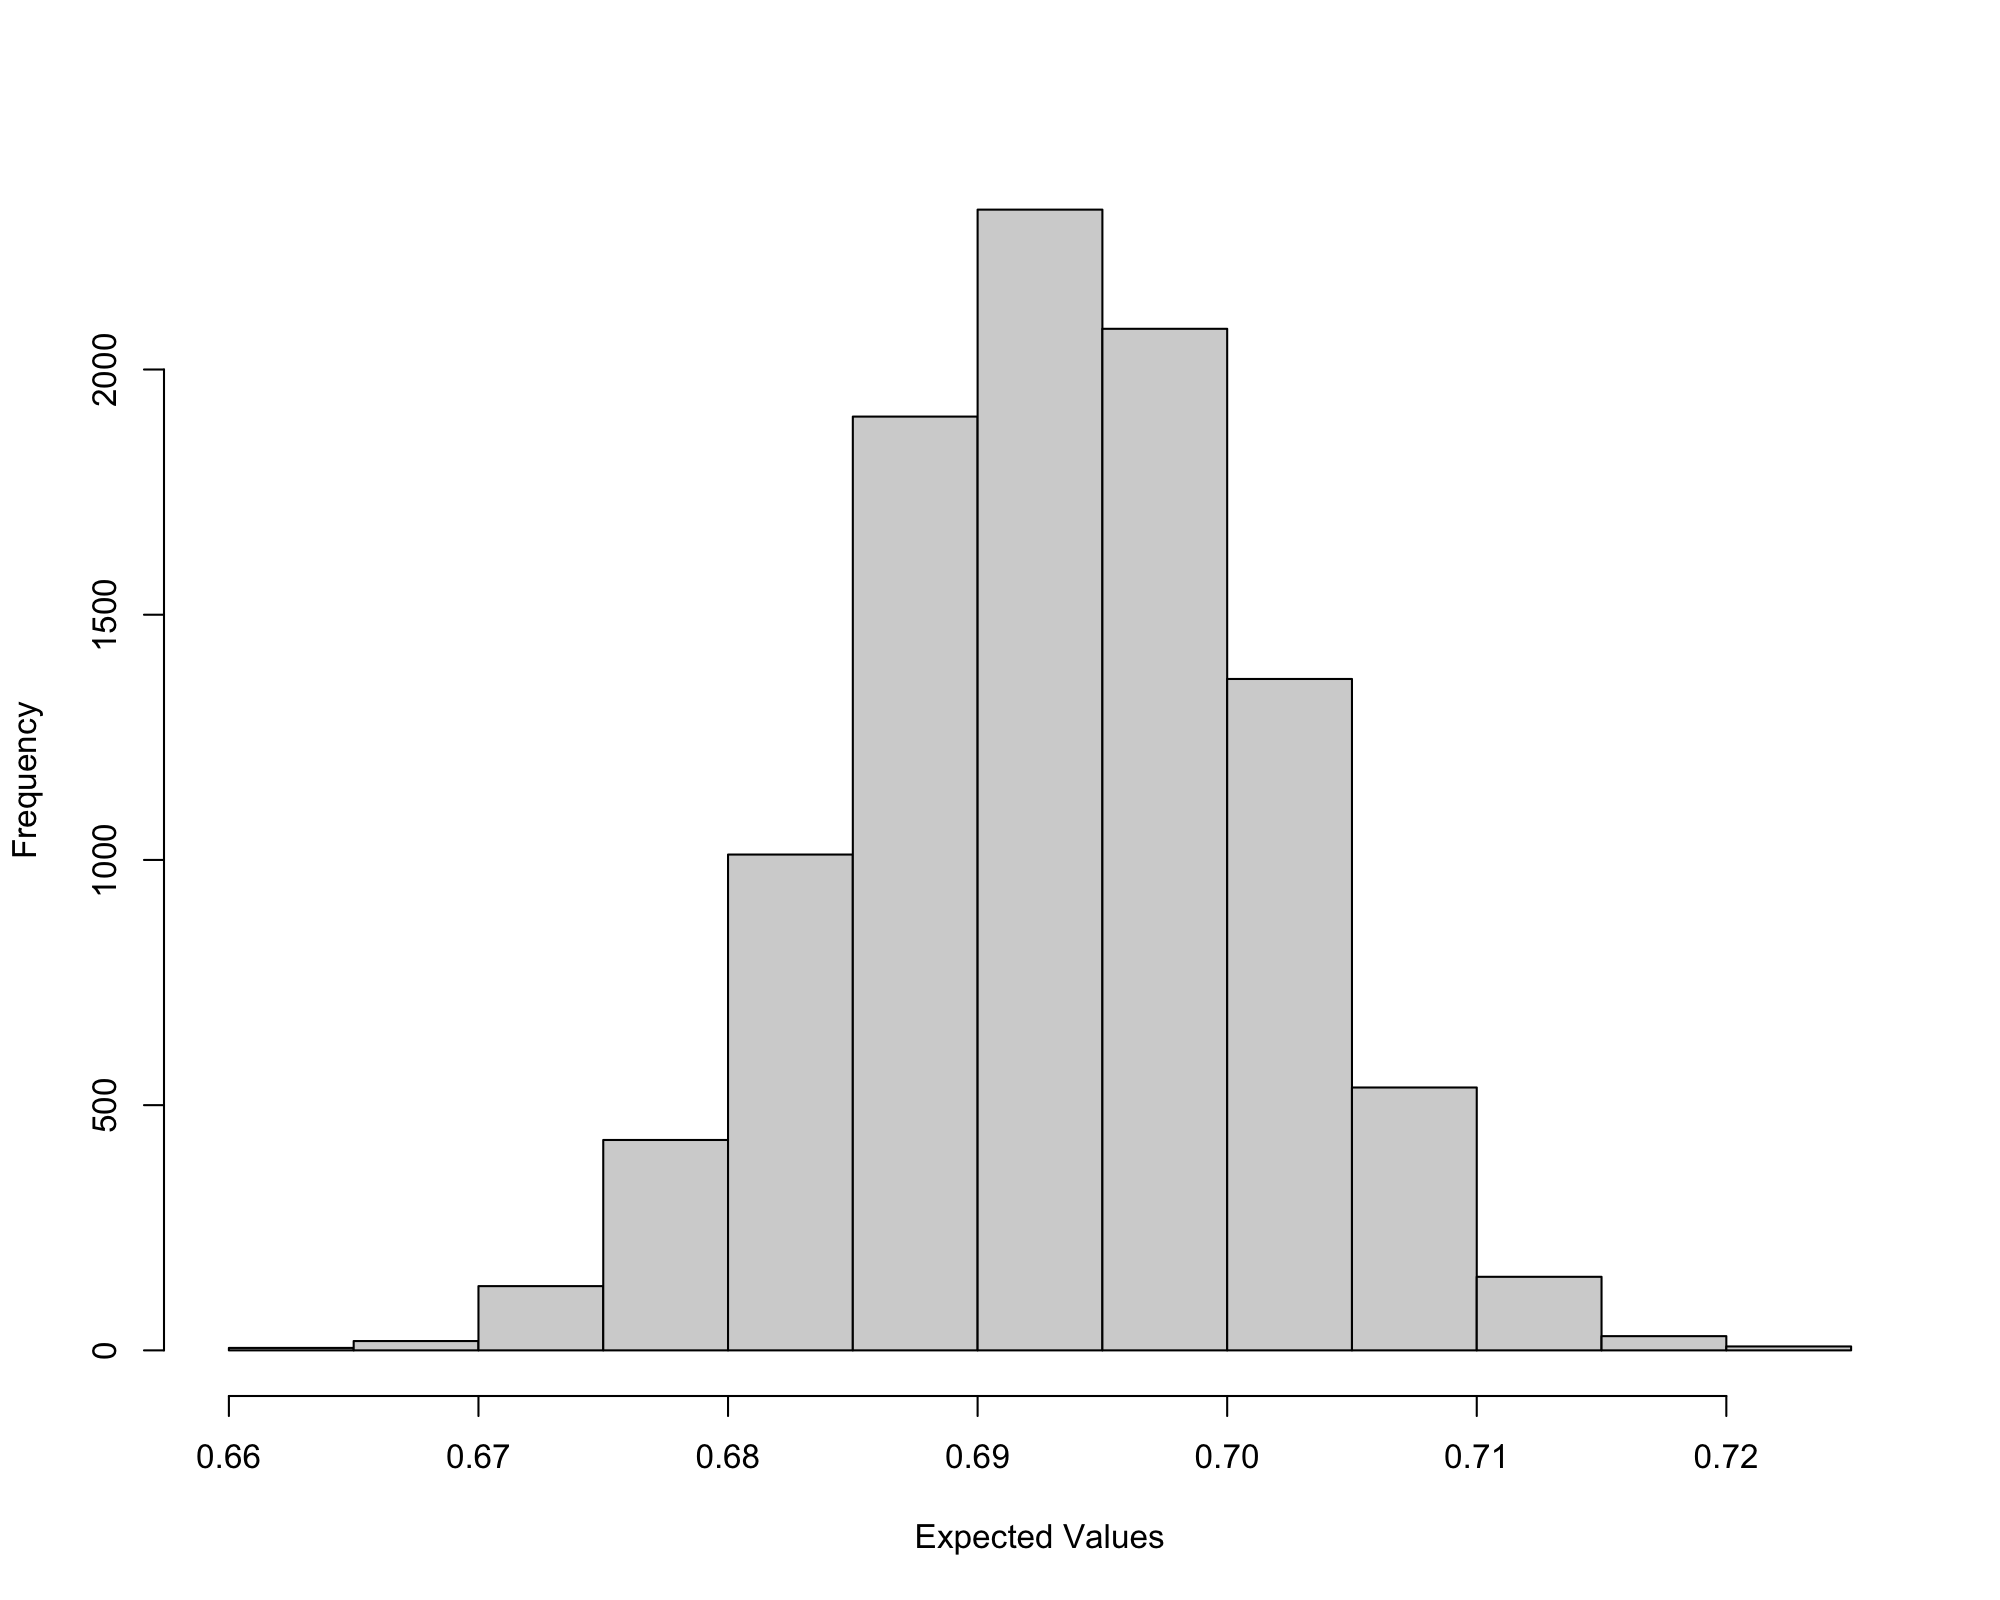
\includegraphics[scale=0.18]{hist}
		\captionof{figure}{Histogram of the simulated expected values in Exercise 12 page 280}
		\label{fig:hist12p280}
	\end{center}
\end{figure}

	\subsubsection*{Exercise 28 page 284}
	
The length of the needle is $ L $ (much bigger than 1). If it is dropped on a grid with a horizontal line, it will form an angle $\theta$ with intersections is $L\cos \theta $ and with a vertical line with intersections is $L\sin \theta $. The uniform probability density function of $\theta$ between $0$ and $\dfrac{\pi}{2} $ is:
$$ \begin{cases}
	\dfrac{2}{\pi}
	& \mbox{if $0\leq \theta \leq  \dfrac{\pi}{2}$,}\\
	0 & \mbox{elsewhere.} \end{cases}
$$
Therefore the average number of lines crossed approximately is:
\begin{equation*}
	\begin{aligned}
	a &	= \dfrac{2}{\pi} \int_{0}^{\frac{\pi}{2}} L \left( cos\theta + sin\theta\right] d\theta \\
	 &	= \dfrac{2L}{\pi} \left[ sin\theta - cos\theta\right]_{0}^{\frac{\pi}{2}} \\
	 &	= \dfrac{4L}{\pi}. \\
	\end{aligned}	
\end{equation*}
		
\clearpage

	\bibliography{tarea9}
	\bibliographystyle{plainnat}
	
\end{document}